\section{Fasövergångar}
Ett ämnes faser eller \emph{aggregationstillstånd} är det olika konfigurationer som dess materia kan anta. I de allra flesta fall finns det tre faser av materia men i vissa omständigheter finns det fyra. De främsta tre kommer täckas av denna kurs men det är bra att veta om den fjärde också. Fasernas namn och namn på övergångarna mellan de är som följande:
\begin{center}
    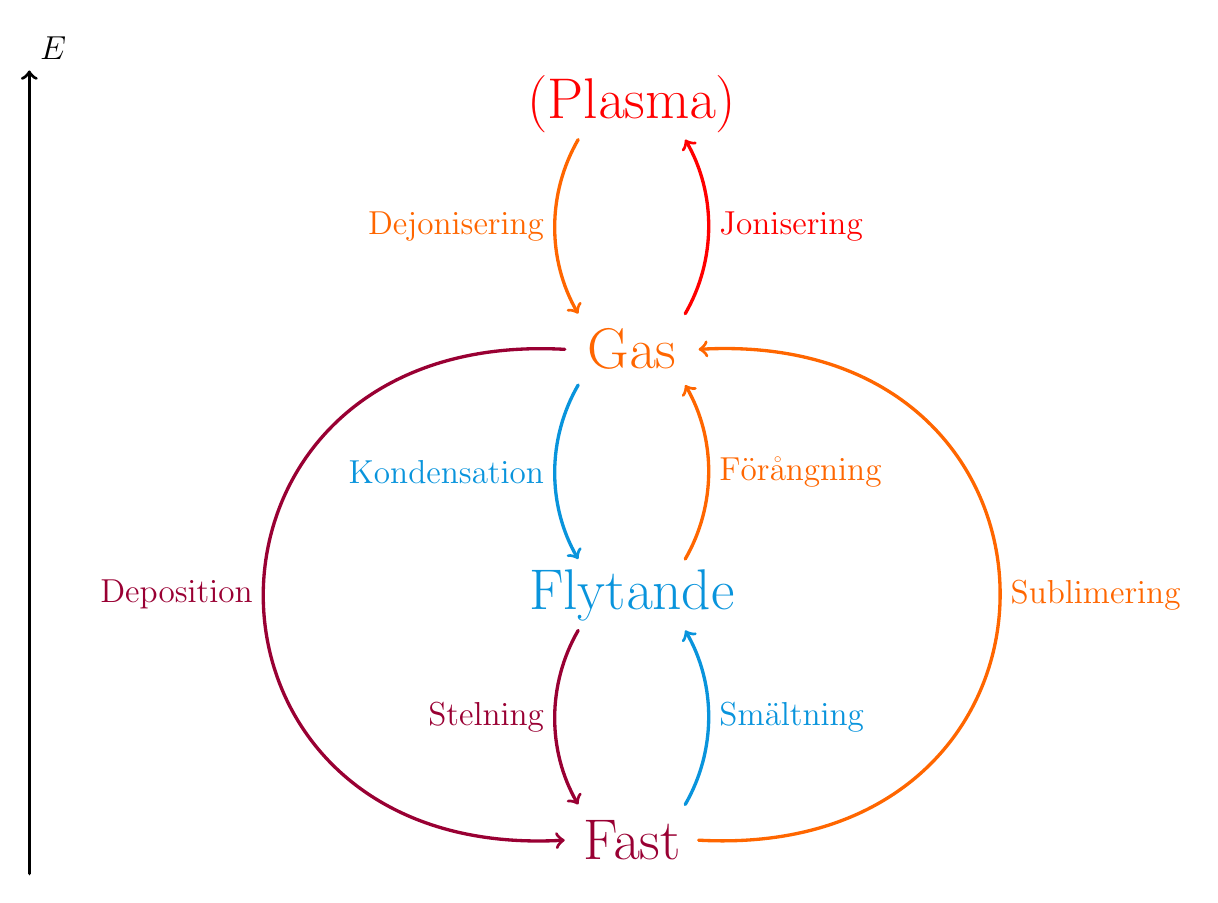
\begin{tikzpicture}[every path/.style={line cap=round, very thick}, scale=0.85]
        \draw[->] (-9,-6) -- ++(0,12) node [anchor=south west] {\large{$E$}};
        %Phases
        \node[color=purple!80!black] at (0,-5.5) {\huge{Fast}};
        \node[color=cyan!80!blue] at (0, -11/6) {\huge{Flytande}};
        \node[color=orange!80!red] at (0, 11/6) {\huge{Gas}};
        \node[color=red] at (0, 5.5) {\huge{(Plasma)}};
        %transitions up
        \draw[->, yshift=-1.3cm, xshift=0.8cm, color=cyan!80!blue] (0,-11/3) arc [radius=2.6cm,start angle=330, delta angle=60] node [pos=0.5, anchor=west, align=left] {\large{Smältning}};
        \draw[->, yshift=-1.3cm, xshift=0.8cm, color=orange!80!red] (0,0) arc [radius=2.6cm,start angle=330, delta angle=60] node [pos=0.5, anchor=west, align=left] {\large{Förångning}};
        \draw[->, yshift=-1.3cm, xshift=0.8cm, color=red] (0,11/3) arc [radius=2.6cm,start angle=330, delta angle=60] node [pos=0.5,anchor=west,align=left] {\large{Jonisering}};
        %Transitions down
        \draw[<-, yshift=-1.3cm, xshift=-0.8cm, color=purple!80!black] (0,-11/3) arc [radius=2.6cm,start angle=210, delta angle=-60] node [pos=0.5, anchor=east, align=right] {\large{Stelning}};
        \draw[<-, yshift=-1.3cm, xshift=-0.8cm, color=cyan!80!blue] (0,0) arc [radius=2.6cm,start angle=210, delta angle=-60] node [pos=0.5, anchor=east, align=right] {\large{Kondensation}};
        \draw[<-, yshift=-1.3cm, xshift=-0.8cm, color=orange!80!red] (0,11/3) arc [radius=2.6cm,start angle=210, delta angle=-60] node [pos=0.5,anchor=east,align=right] {\large{Dejonisering}};
        %full range transitions
        \draw[->, color=orange!80!red] (1,-5.5) .. controls (7,-11/6-4) and (7,-11/6+4) .. (1,11/6) node [pos=0.5,align=left,anchor=west] {\large{Sublimering}};
        \draw[<-, color=purple!80!black] (-1,-5.5) .. controls (-7,-11/6-4) and (-7,-11/6+4) .. (-1,11/6) node [pos=0.5,align=right,anchor=east] {\large{Deposition}};
    \end{tikzpicture}
\end{center}
\subsection*{Plasma}
En mycket var joniserad gas. Hittas exempelvis i stjärnor. Täcks inte av krusen.
\subsection*{Gas}
När de olika formelenheterna av ämnet är i princip obundna till varandra och kan flyta fritt i omgivningen. Detta aggregationstillstånd har högst inre rörelseenergi.
\subsection*{Flytande}
Detta tillstånd, bättre känt som vätska, är det som händer när formelenhetern är löst bundna till varandra. Detta gör att de kan röra på sig occh anpassa sin form för att passa behållaren men är inte lika fria som en gas. Den viktigaste skillnaden är dock att vätskor är okomprimerbara till skillnad från gaser.
\subsection*{Fast}
Detta är när formelenheterna är hårt bundna till varandra är helt orörliga. Det finns många olika sätt att kunna anta fast form. Vissa ämnen bildar kristaller, andra metallbinder bland annat.